\subsection{Gameplay}

\subsubsection{Système de verrouillage}

Pour tuer un personnage (joueur ou NPC),
nous avons ajouté un système de verrouillage. Celui-ci est assez pratique : lorsque l'on passe dans ce mode, l'écran change et 
un effet réalisé grâce au post processing de Unity permet de donner un effet sépia/vieux films\footnote{voir Effets Graphiques}.
Un contour blanc autour des personnages visés au centre de l'écran permettent voir quel personnage va être sélectionné.

Une fois sa cible sélectionnée, le joueur peut l'éliminer à condition d'en être suffisamment proche.

L'effet a demandé de créer plusieurs overlays de caméra, afin d'avoir un effet graphique
appliqué uniquement sur certains layers, et de les surperposer les uns sur les autres. 

\subsubsection{Finishers}
Nous avons fourni un vrai travail sur les différentes animations de mort des personnages.
Lors de sa réalisation, un problème s'est posé : Il fallait que les animations de deux GameObject (ici le joueur qui tue et le NPC/joueur tué) 
soient parfaitement synchronisées. Après avoir regardé plusieurs types de solutions, nous nous sommes tournés vers un outil préintégré appelé Timeline.
Ce dernier permet de réaliser des clips vidéos.

Voici donc comment nous avons intégré les timelines :
\newline
Des faux personnages jouant les animations sont ajoutés sur la carte à la position et rotation du tueur.
On masque le tueur et la victime de la carte.
On change le mesh et le matériau de chaque personnage de la timeline pour qu'il corresponde au tueur et au
personnage tué.

Une fois l'animation terminée, un signal est envoyé à un script qui réaffiche alors le joueur qui était masqué.
Si le personnage tué était un joueur, alors il réapparait discrètement ailleurs sur la map lors de sa réaparition.
Le personnage tué disparait de la carte au bout d'une dizaine de secondes avec un shader fait avec Shader Graph.

Voici quelques finishers que nous avons réalisé :

\begin{figure}[hbt!]
    \centering
    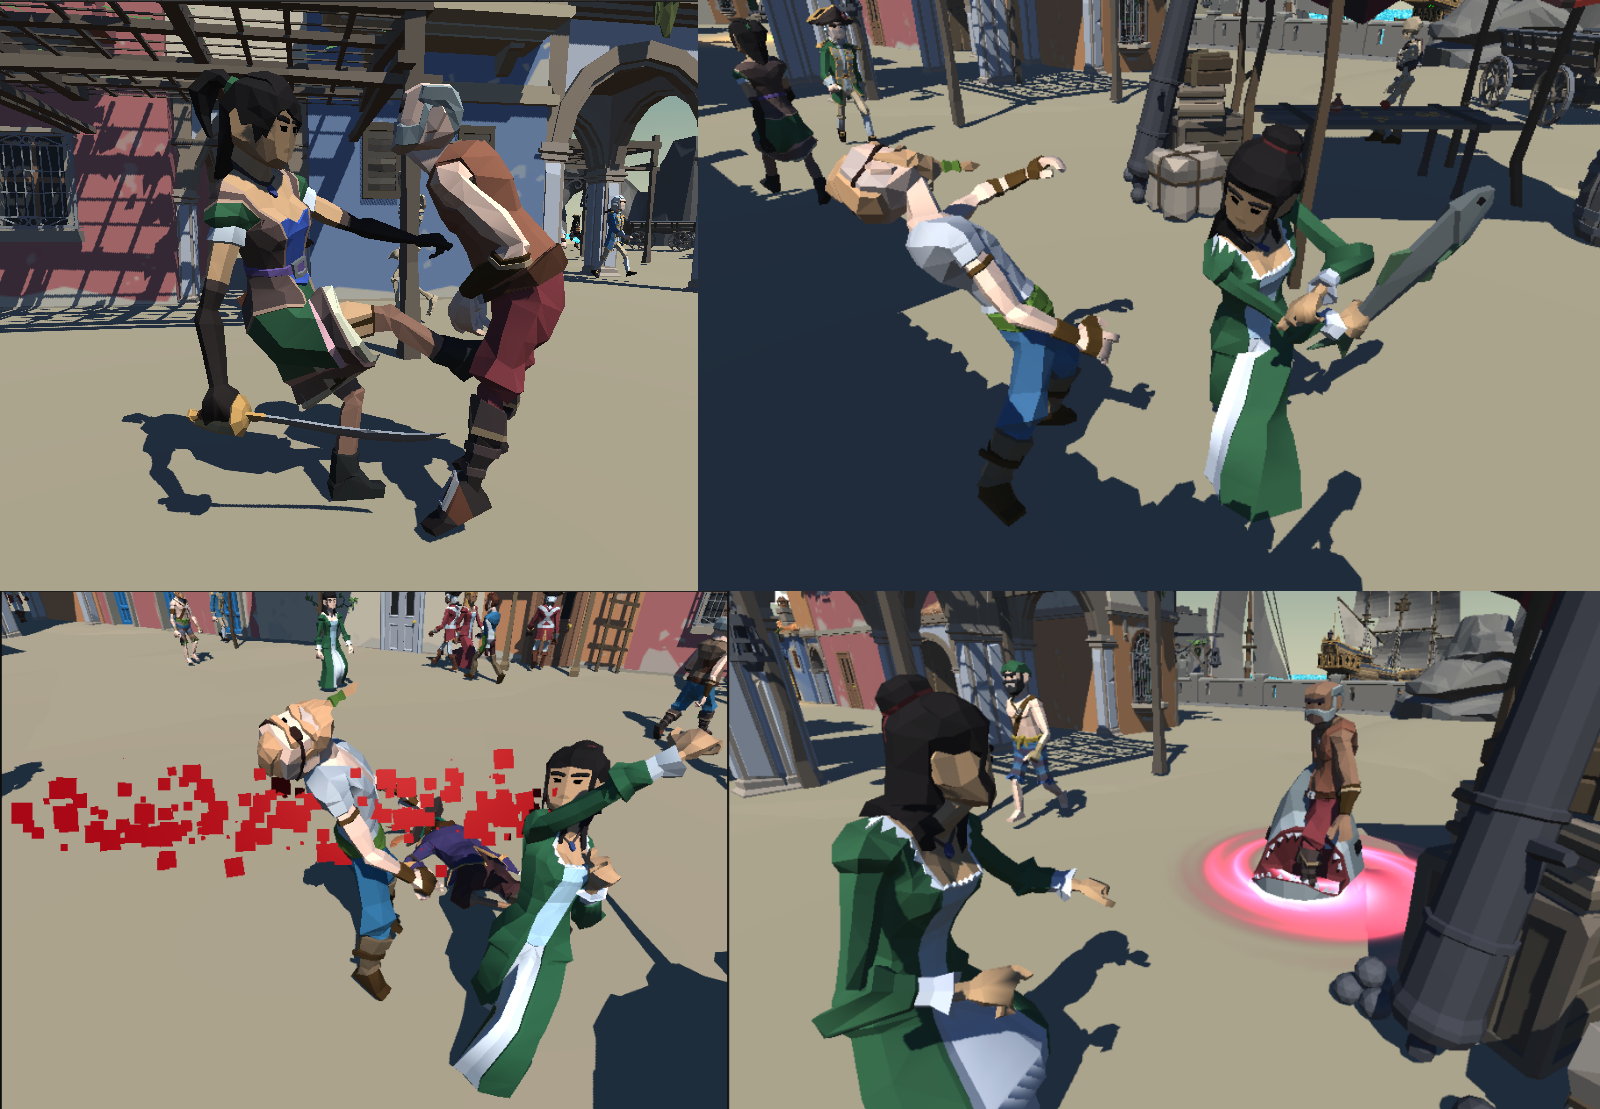
\includegraphics[scale=0.27]{finishers/finishers.png}
    \caption{Quelques finishers}
\end{figure}

\FloatBarrier
\begin{figure}[hbt!]
    \centering
    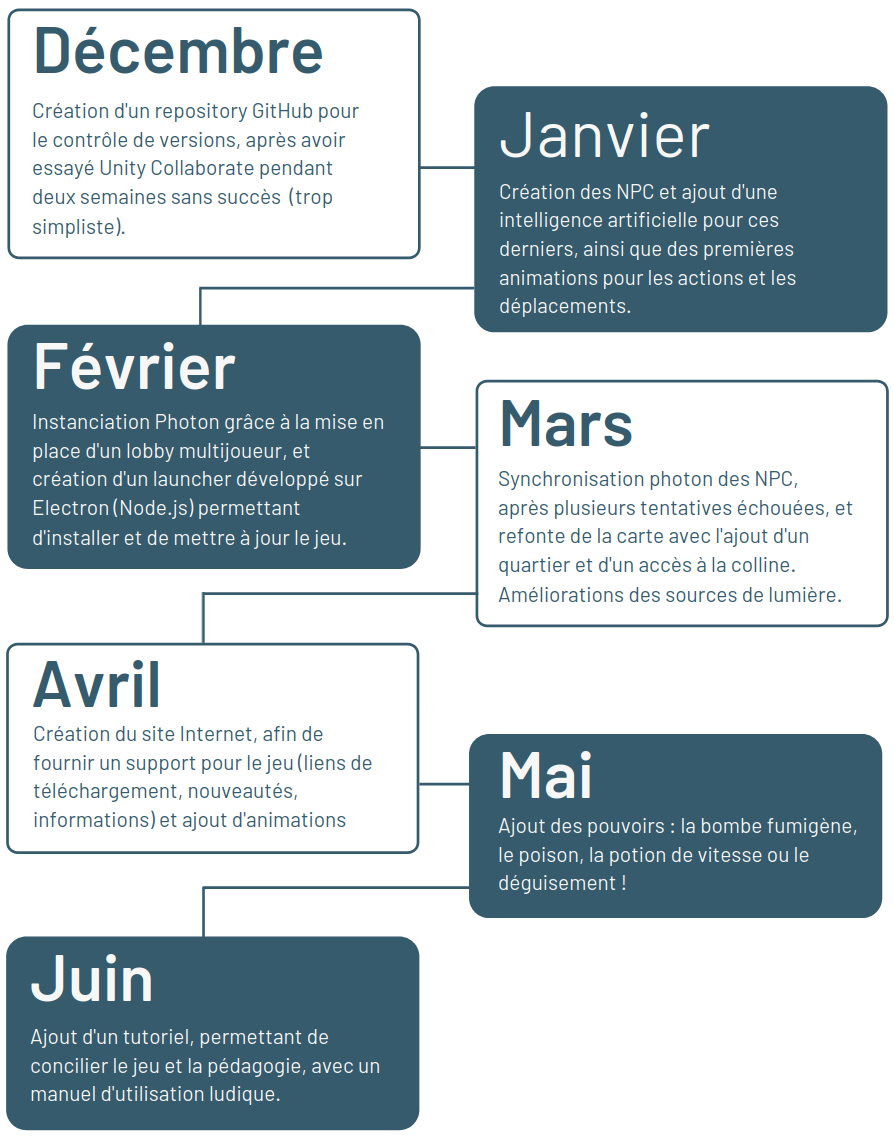
\includegraphics[scale=0.3]{timeline.png}
    \caption{Timeline du lancer de hache}
\end{figure}


\subsubsection{Système de manche}
    Le système actuellement utilisé pour le déroulement d'une partie se base sur des manches. Le jeu se fait en deux phases:
    	-Une période de 'grâce' de 30 secondes où les joueurs attendent l'assignation d'une cible. 
	 Ils sont libres de se déplacer, pour se cacher par exemple.

	-Une période de 'chasse'. Les cibles sont assignées et le combat peut commencer. Elle est au départ de 3 minutes, mais ce temps
	 diminue à chaque mort de joueur pour pousser les participants au meurtre.

\subsubsection{Système de mort}
    Joueurs comme IA peuvent être tués. Dans le cas d'un joueur, un système de mort a été mis en place. Ainsi,
    quand le joueur se fait tuer, son personnage est désactivé temporairement et il rentre
    en mode "spectateur". Il peut se balader sur la map, mais il ne peut en aucun cas interagir avec l'environnement,
	et il n'est pas visible des autres joueurs.

\subsubsection{Système de point}
    Un système de point a également été implémenté. Il fonctionne de la façon suivante:
    
	-Tuer sa cible rapporte des points. le premier joueur tuant sa cible gagne plus de point, les autres en gagne de moins en moins.
	
	-Tuer une IA fait perdre des point! Il faut donc faire attention à ne pas tuer n'importe qui. Celà encourage la réflexion et pas simplement un carnage afin de trouver sa cible.
	
	-Tuer la cible de quelqu'un d'autre ne fait pas perdre de points, mais un système de compensation a été mis en place. Ainsi, se faire voler sa cible par un autre joueur apporte des points de compensation. Encore une fois, il n'est donc pas dans l'intérêt 
	des joueurs de tuer le premier venu !

	-Une autre façon de gagner des points et d'être encore en vie à la fin d'une manche.

    Tous ces élémens permettent de déterminer le classement de la partie.
	
\subsubsection{Système de fin de partie}
	Finir une partie est tout un processus. Il faut d'abord désactiver le mouvement des joueurs.
	On présente ensuite plusieurs informations aux joueurs comme leur rang final, le nombre d'assassinats
	et de mort, ainsi que l'expérience acquise. Ensuite, on propose au joueur de rejouer. S'il refuse, il quitte la salle.
	Sinon, quand tout les joueurs ont fait leur choix, ils retournent sur le lobby dans l'attente d'une prochaine partie.

\subsubsection{Cinemachine}